\documentclass[xcolor={dvipsnames},pdf, hyperref={colorlinks=true, citecolor=ForestGreen, linkcolor=BlueViolet, urlcolor=Magenta}]{beamer}
\usetheme{Frankfurt}  
\usecolortheme{whale}
\usepackage{tikz} 
\usepackage{graphicx}
\usepackage{dsfont}
\usepackage{hyperref}
\usepackage{alltt}
\usepackage{enumerate}
\usepackage{amsthm}
\theoremstyle{definition}
\newtheorem{exmp}{Example}[section]
\usepackage{verbatim}               % useful for \begin{comment} and \end{comment}
\usepackage{eurosym}                % used for euro symbol
\usepackage{caption} 
\usepackage{graphicx}
\usepackage{adjustbox}
\graphicspath{{Figures/}}
\usepackage{subcaption}
\usepackage{color}
\usepackage{float}
\usepackage{amssymb}
\usepackage{MnSymbol,wasysym}
\usepackage{sgamevar}
\usepackage{remreset}% tiny package containing just the \@removefromreset command
\makeatletter
\@removefromreset{subsection}{section}
\makeatother
\setcounter{subsection}{1}



\newcommand{\defn}[1]{\textbf{#1}}


%Instructor version
\newcommand{\blank}[0]{}
\newcommand{\ddp}[1]{{\textcolor{ForestGreen}{#1}}} 
\newcommand{\dd}[1]{{\underline{\textcolor{ForestGreen}{#1}}}}

%Student version
%\newcommand{\blank}[0]{\vspace{2em}}
%\newcommand{\dd}[1]{\underline{\hspace{3cm}}} 
%\newcommand{\ddp}[1]{}

\addtobeamertemplate{navigation symbols}{}{%
	\usebeamerfont{footline}%
	\usebeamercolor[fg]{footline}%
	\hspace{1em}%
	\insertframenumber/\inserttotalframenumber
}

\section{The Business Cycle}

%% preamble
\title{Aggregate Demand and Supply}
\author{David A. D\'iaz}
\institute{UNC Chapel Hill}
\date{}

\AtBeginSection[] %Section links on slides

\begin{document} 
	
	\begin{frame}
		
		\titlepage
		
	\end{frame}

\begin{frame}{Economic Fluctuations}
\begin{itemize}
	\item Short-run GDP fluctuations in the economy are called the \dd{business cycle}. 
	\item During periods of \dd{expansion}, real GDP \dd{increases} and firm profits are \dd{growing}.
	\item Conversely, during periods of economic \dd{recession}, real GDP \dd{falls} and firm profits are \dd{decreasing}.
	\item A main point to remember about the business cycle is that economic fluctuations are \dd{irregular} and largely \dd{unpredictable}.
\end{itemize}
\end{frame}

\begin{frame}{Economic Fluctuations}
	\begin{itemize}
		\item Additionally, most macroeconomic quantities tend to fluctuate \dd{together} in the short run (e.g., real GDP, personal income, consumer spending, etc.). 
		\item However, what does differ is the \dd{magnitude} of the fluctuations.
		\item Finally, as real GDP output falls, the rate of unemployment \dd{increases}. 
	\end{itemize}
\end{frame}

\begin{frame}{Economic Fluctuations}
	\begin{itemize}
		\item Recall that according the classical theory, changes in the money supply only affect \dd{nominal} variables, but not \dd{real} variables. 
		\item We noted that this only describes the world in the long run, but not in the short run.
		\item  In the short run, money is \textbf{not} neutral because real and nominal variables are heavily related in this period. 
	\end{itemize}
\end{frame}

\section{Aggregate Demand}

\begin{frame}{Aggregate Demand}
	\begin{itemize}
		\item The aggregate demand curve shows combinations of \dd{inflation} and \dd{real GDP growth} that make up a certain rate of \dd{spending growth}. 
		\item Spending growth comes from household, firm, and government purchases as well as money growth ($\vec{M} + \vec{v}$). 
		\item From the Quantity Equation (expressed in percent change terms),  \[\vec{M} + \vec{v} = \pi + \vec{Y}\] 
	\end{itemize}
\end{frame}


\begin{frame}{Aggregate Demand}
	\begin{itemize}
		\item Shifts in the AD curve can arise from any of the following:
		\begin{enumerate}
			\item Changes in consumption spending
			\item Changes in investment spending
			\item Changes in government purchases
			\item Changes in net exports
			\item Changes in the money supply
		\end{enumerate}
	\item Any shock that affects (1) - (4) (e.g., a rise in consumer or business optimism) is referred to as an \dd{aggregate demand shock}.
	\end{itemize}
\end{frame}


\begin{frame}{Aggregate Demand}

\begin{figure}[H]
	\centering
	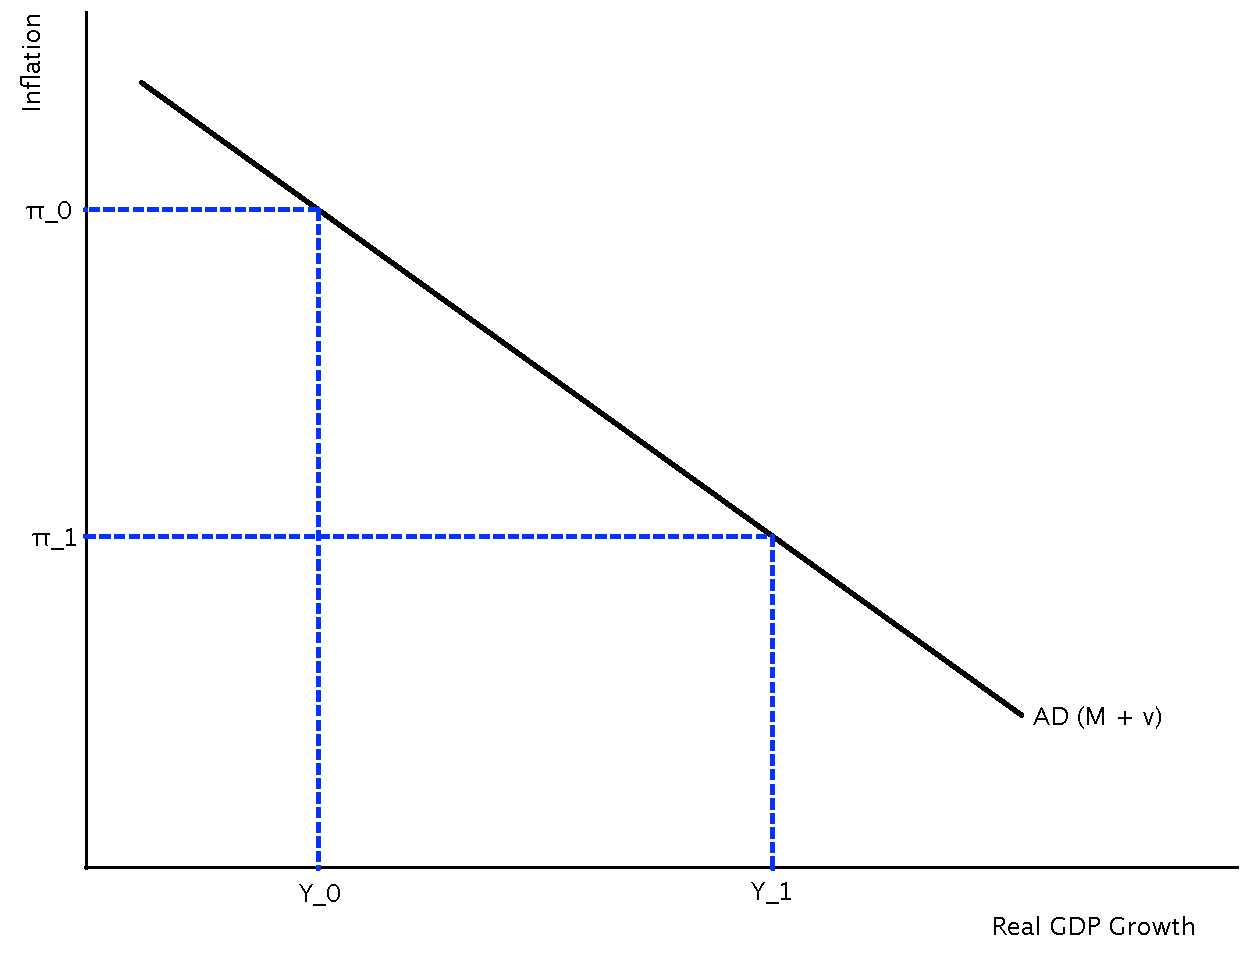
\includegraphics[scale=.40]{plot95.pdf}
	\caption{Aggregate Demand Curve}
	
\end{figure}

\end{frame}

\begin{frame}{Aggregate Demand}
\begin{exmp}
	If the velocity of money is constant, what is the growth rate of the money supply in the economy if spending growth is 5\%? If the Fed increased the money supply so that the money growth rate was 7\%, what would be the effect on the aggregate demand curve?
\end{exmp} 
\end{frame}

\begin{frame}{Aggregate Demand}
\begin{figure}[H]
	\centering
	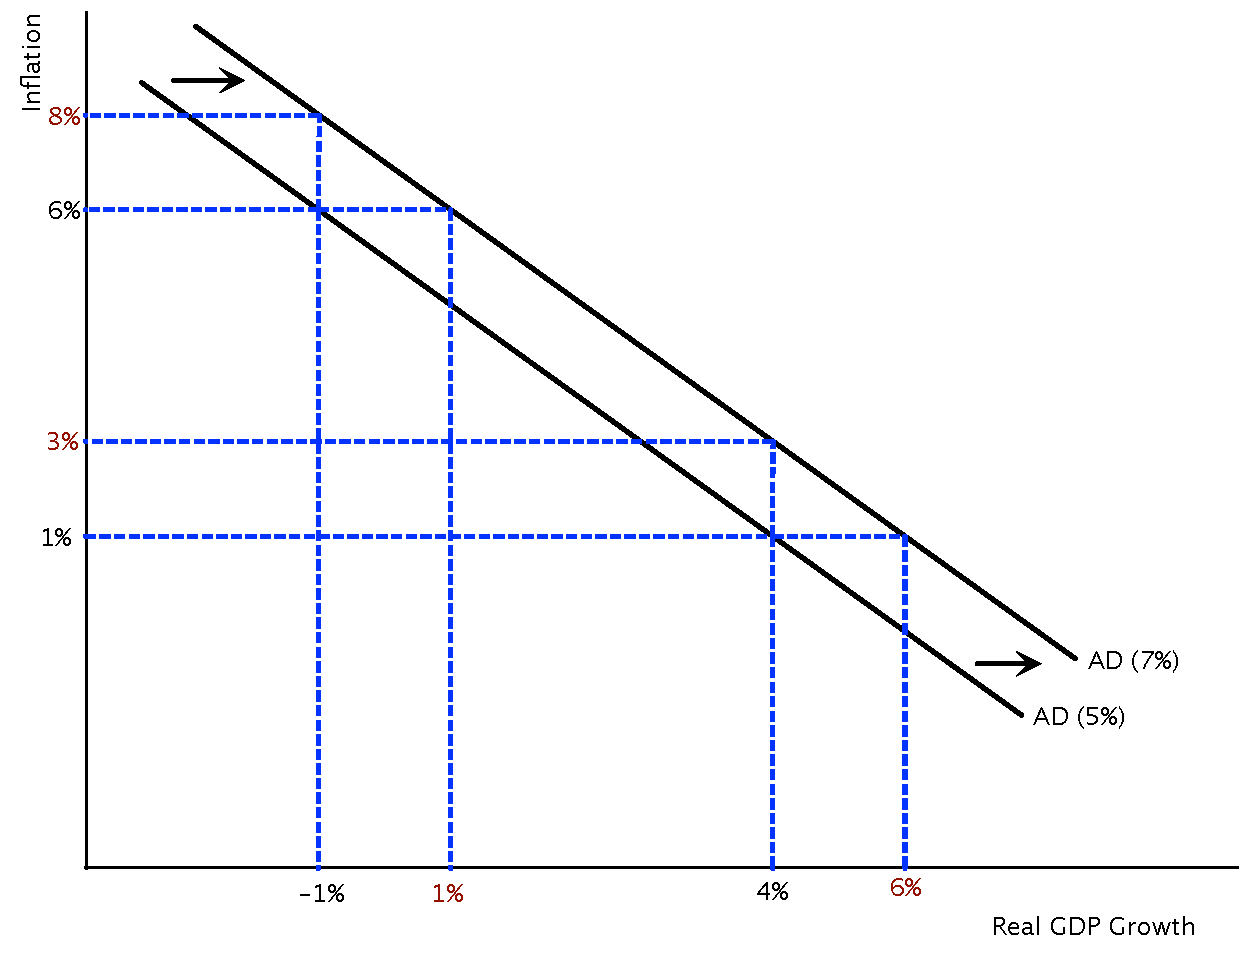
\includegraphics[scale=.40]{plot96.pdf}
	\caption{AD Shifts}
\end{figure}
\end{frame}

\section{Aggregate Supply}

\begin{frame}{Aggregate Supply}
	\begin{itemize}
		\item The AS curve comes from the quantity of goods and services that firms choose to produce and sell.
		\item The AS curve has two representations - the \dd{long-run} AS curve and the \dd{short-run} AS curve. 
		\item In the long run, an economy's production of goods and services depends on  its supply of
		\begin{enumerate}
			\item Labor
			\item Capital
			\item Natural resources
			\item Available technology
		\end{enumerate}
	\end{itemize}
\end{frame}

\begin{frame}{Aggregate Supply}
	\begin{itemize}
		\item Because in the long run, money is neutral, the inflation rate has \dd{no} effect on the growth rate of real GDP. 
		\item Thus, the LRAS curve is \dd{vertical} and the rate of real GDP growth in the long run is referred to as the \dd{natural (solow) rate} of GDP growth.
		\item Shifts in the LRAS come about due to any changes in (1) - (4), and these shocks are called \dd{real} shocks (e.g., new inventions, increases in the price of oil, etc.).
	\end{itemize}
\end{frame}

\begin{frame}{Aggregate Supply}
	\begin{itemize}
		\item On the otherhand, the SRAS curve is \dd{upward-sloping}. 
		\item That is, the inflation rate in an economy does have an effect on the growth rate of real output in the short run.
		\item The reason this is the case is due to expectations of inflation mismatching reality. When the inflation rate is above what people expect, output growth rises \dd{faster} than its natural rate, and vice-versa. 
	\end{itemize}
\end{frame}

\begin{frame}{Aggregate Supply}
	\begin{itemize}
		\item Two theories that explain this:
		\begin{enumerate}
			\item Sticky wages: Nominal wages are slow to adjust to changing conditions. Thus, when prices increase firm profits increase, leading them to increase production $\Rightarrow Y$ increases. Eventually, workers renegotiate wages and nominal wages increase.
			\item Sticky prices: Prices are slow to adjust. Example: An unexpected fall in prices leads some firms to have higher-than-desired prices, which decreases sales and thus firms reduce output $\Rightarrow$ GDP falls.
		\end{enumerate}
	\end{itemize}
\end{frame}


\begin{frame}{Aggregate Supply}
	\begin{figure}[H]
	\centering
	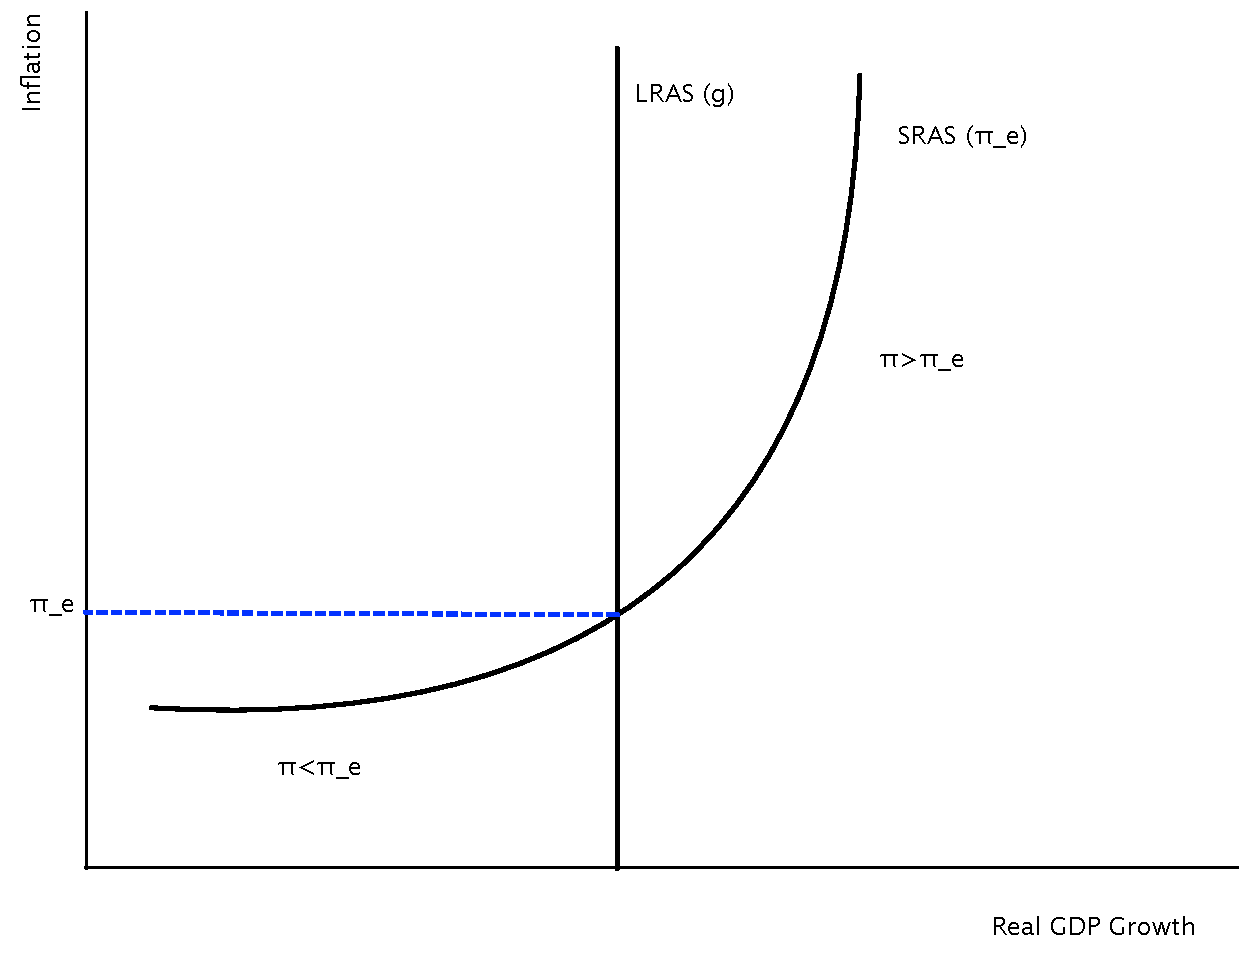
\includegraphics[scale=.40]{plot97.pdf}
	\caption{LRAS and SRAS}
\end{figure}
\end{frame}

\begin{frame}{Aggregate Supply}
	\begin{itemize}
		\item The SRAS is steeper to the right of $g$ because an economy can only grow so fast. Because wages are more sticky in the downward direction, the SRAS curve is flatter to the left of $g$.
		\item Since the SRAS curve reflects expectations about the inflation rate in the economy, shifts are caused by changes in the \dd{expected inflation rate}.
	
		
	\end{itemize}
\end{frame}


\begin{frame}{Aggregate Supply}
\begin{itemize}

	\item Specifically, when the expected inflation rate increases, the SRAS curve shifts \dd{upward (to the left)}, and when the expected inflation rate decreases, the SRAS curve shifts \dd{downward (to the right)}.
	\item The expected inflation rate of a given SRAS curve is given by the \dd{intersection} of the SRAS and LRAS curves.
	
\end{itemize}
\end{frame}
\section{The AS-AD Model}


\begin{frame}{AS-AD}
	
	\begin{figure}[H]
		\centering
		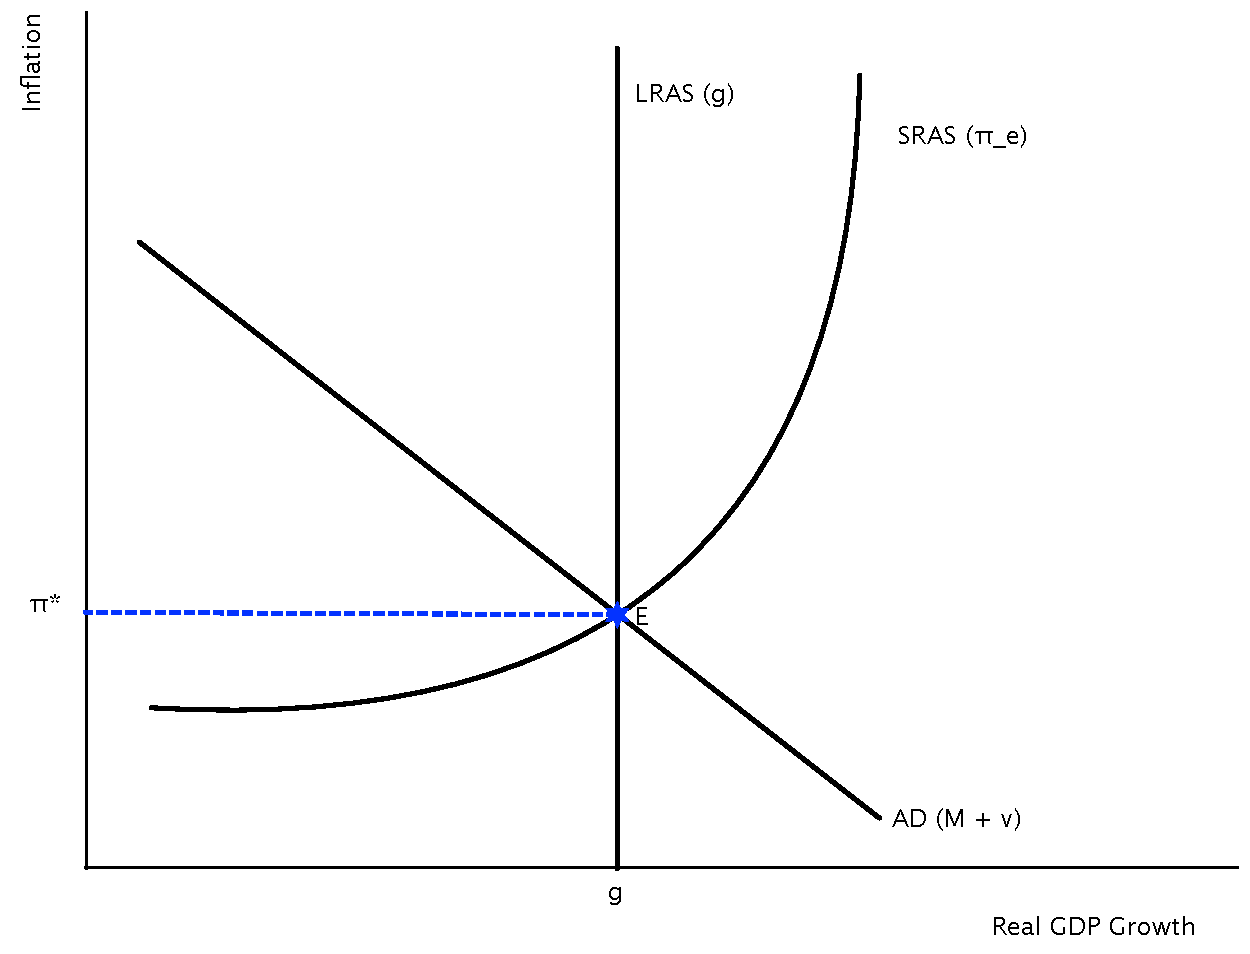
\includegraphics[scale=.35]{plot98.pdf}
		\caption{Long-Run Equilibrium}
	\end{figure}
	

\end{frame}


\begin{frame}{AS-AD}
\begin{itemize}
	\item The long-run equilibrium is given by where the AD curve and the LRAS curve intersect. 
	\item When the economy reaches point $E$, the expected inflation rate has adjusted to the long-run inflation rate and thus the SRAS curve crosses this point as well.
\end{itemize}
\end{frame}


\begin{frame}{AS-AD}



\begin{figure}
	\centering
		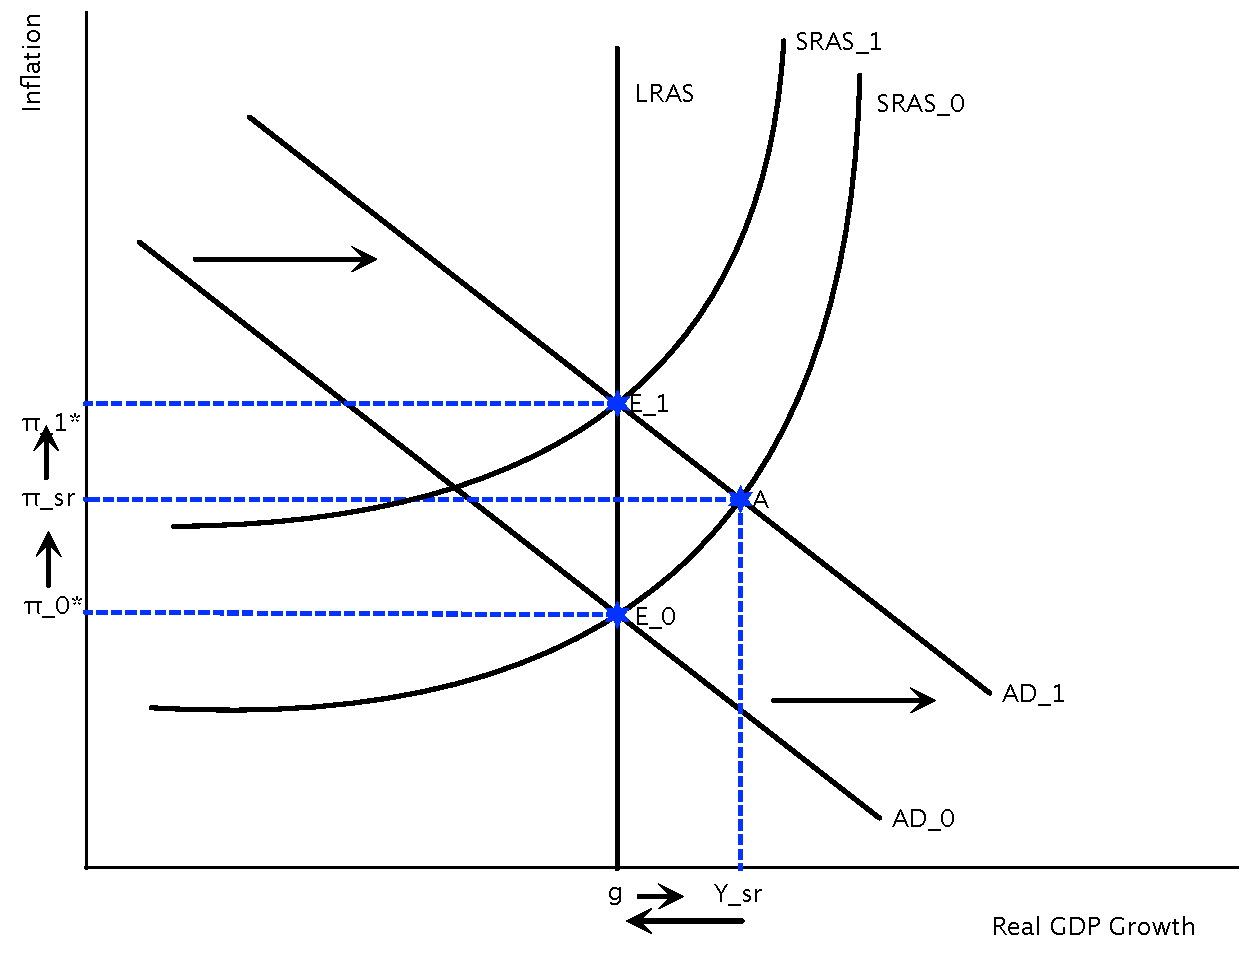
\includegraphics[scale=.35]{plot99.pdf}
		\caption{AD Shock}

\end{figure}

\end{frame}

\begin{frame}{AS-AD}
\begin{figure}
	\centering
	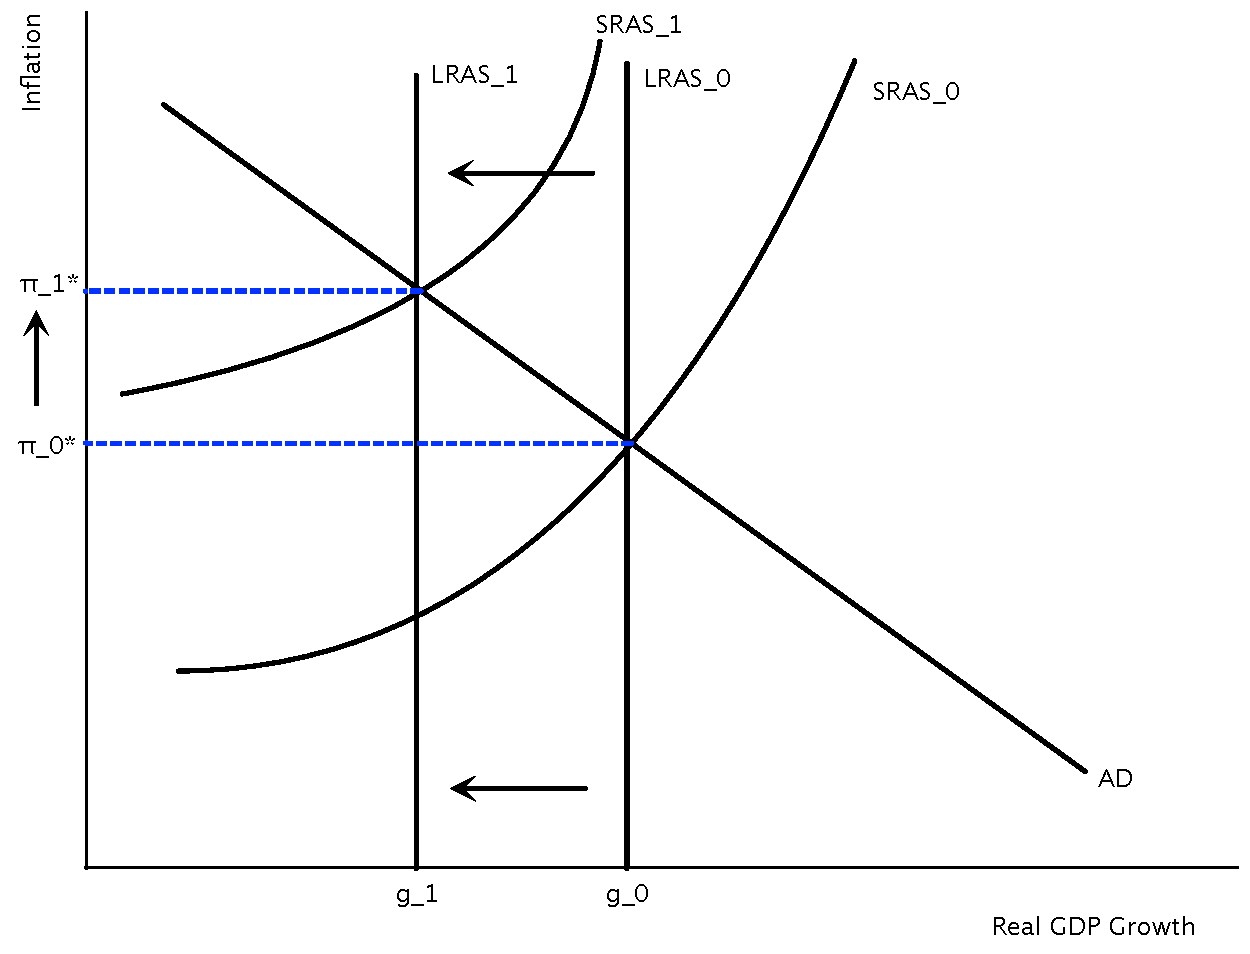
\includegraphics[scale=.35]{plot100.pdf}
	\caption{Real Shock}
\end{figure}
\end{frame}

\begin{frame}{AS-AD}
\begin{exmp}
	Suppose an economy experiences a permanent drop in consumption growth due to declining consumer confidence. How does this change in consumption growth affect the inflation rate and the real GDP growth rate in the short run? In the long run?
\end{exmp}
\end{frame}

\begin{frame}[b]{AS-AD}


\begin{figure}[H]
	\centering
	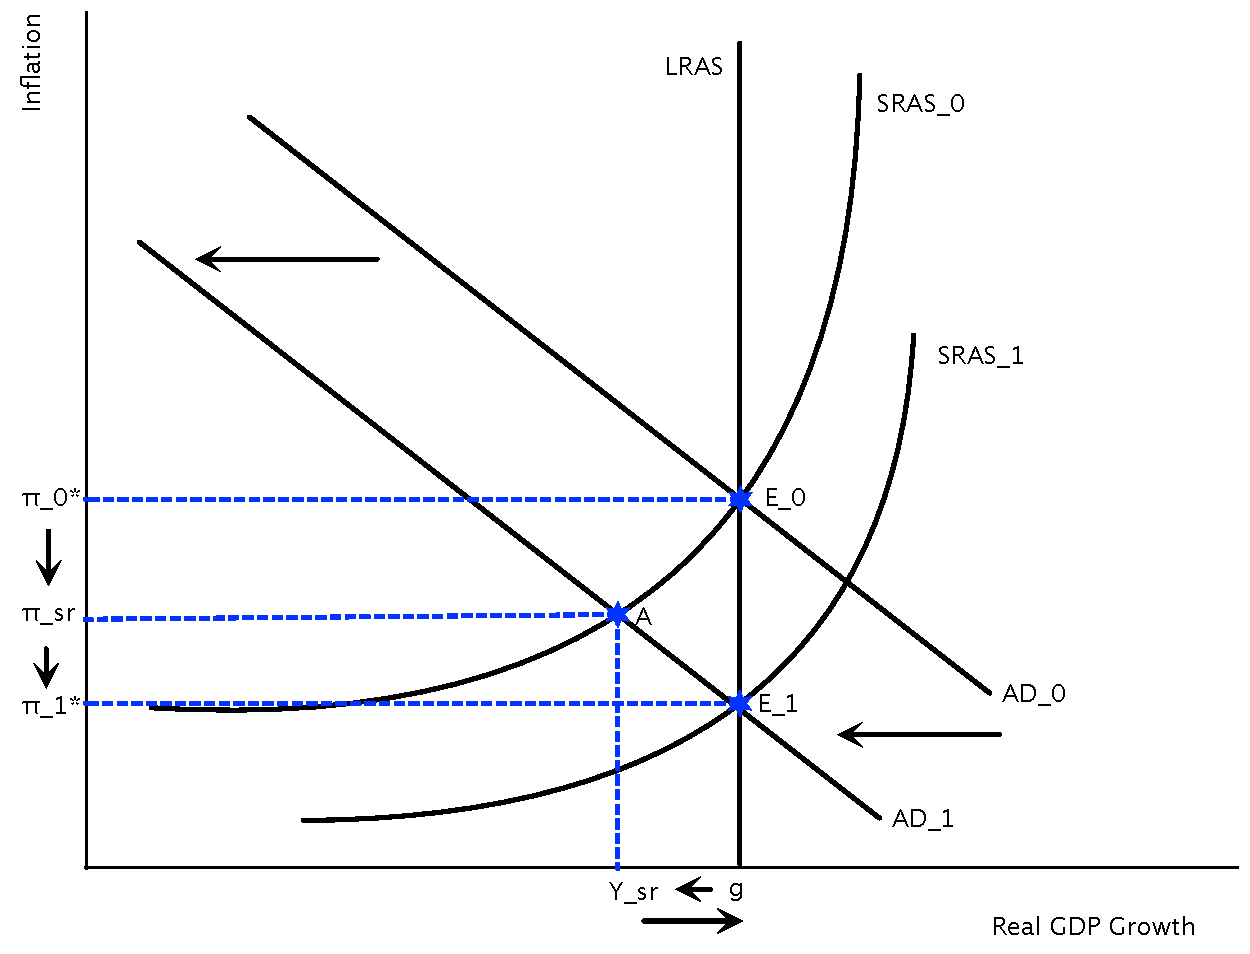
\includegraphics[scale=.40]{plot101.pdf}
	\caption{Example}
\end{figure}

\end{frame}

\begin{frame}{Readings and Assignments}
\begin{itemize}
	\item Today: Mankiw Ch. 33
	\item Next time: Mankiw Ch. 34
	\item Problem Set 6, section 3
\end{itemize}
\end{frame}

\end{document}